\chapter{Methodology}

This project takes a mixed-method approach to investigate the influence of culture on Human-Robot Interaction (HRI), with a focus on national identity as a case study through which to explore cultural differences. The choice to examine cultural impacts through national identity is driven by the distinct and observable characteristics that are deeply rooted within this framework, such as language, social norms, and symbols. These aspects are readily identifiable and offer a strong foundation for designing interaction scenarios that can be systematically evaluated. This approach aims to provide insights into the broader field of cultural adaptability in robotics by studying interactions within the context of a diverse and tangible element of culture — nationality. The methodology comprises a combination of pre-experiment surveys to understand participants' cultural backgrounds and expectations, culturally infused interaction scenarios within a simulated environment, and post-experiment evaluations to gauge the perceptions and experiences of the participants. These stages are designed to collect both qualitative and quantitative data, allowing for a comprehensive analysis of cultural influences on HRI.

\section{Experimental Design}

\subsection{OfficeBots Environment}

The experiments will utilize the OfficeBots simulation, which enables controlled observations of HRI in an office setting. The environment lends itself to a standardized and repeatable research design.

\subsection{Robot Behaviour Modification and Scenarios}

The study will employ three robots, each assigned a set of behavior modifications corresponding to their "nationality" based on predefined user inputs. These nationalities—China, Hong Kong, and the UK—each present unique cultural considerations for language, proximity etiquette, and hospitality norms.

\subsubsection{Interaction Scenarios}

\begin{enumerate}
    \item \textbf{Language Adaptation:}
    \begin{itemize}
        \item A robot representing China will communicate in Simplified Chinese.
        \item A robot representing Hong Kong will use Traditional Chinese.
        \item A robot representing the UK will interact using British English.
    \end{itemize}
    
    \item \textbf{Cultural Hospitality:}
    \begin{itemize}
        \item Each robot will offer beverages associated with their country (water, Hong Kong-styled milk tea, and English tea), reflecting the cultural norm of drink offerings as a form of hospitality.
    \end{itemize}
    
    \item \textbf{Proximity Norms:}
    \begin{itemize}
        \item Adhering to cultural norms regarding personal space, robots will maintain varying distances when approaching participants, respective to their assigned nationality.
    \end{itemize}
\end{enumerate}

By embedding these scenarios into our research design, we gain valuable insights into how cultural adaptations impact user comfort, engagement levels, and overall perception of the robot’s social intelligence.

\begin{figure}
    \begin{center}
        \noindent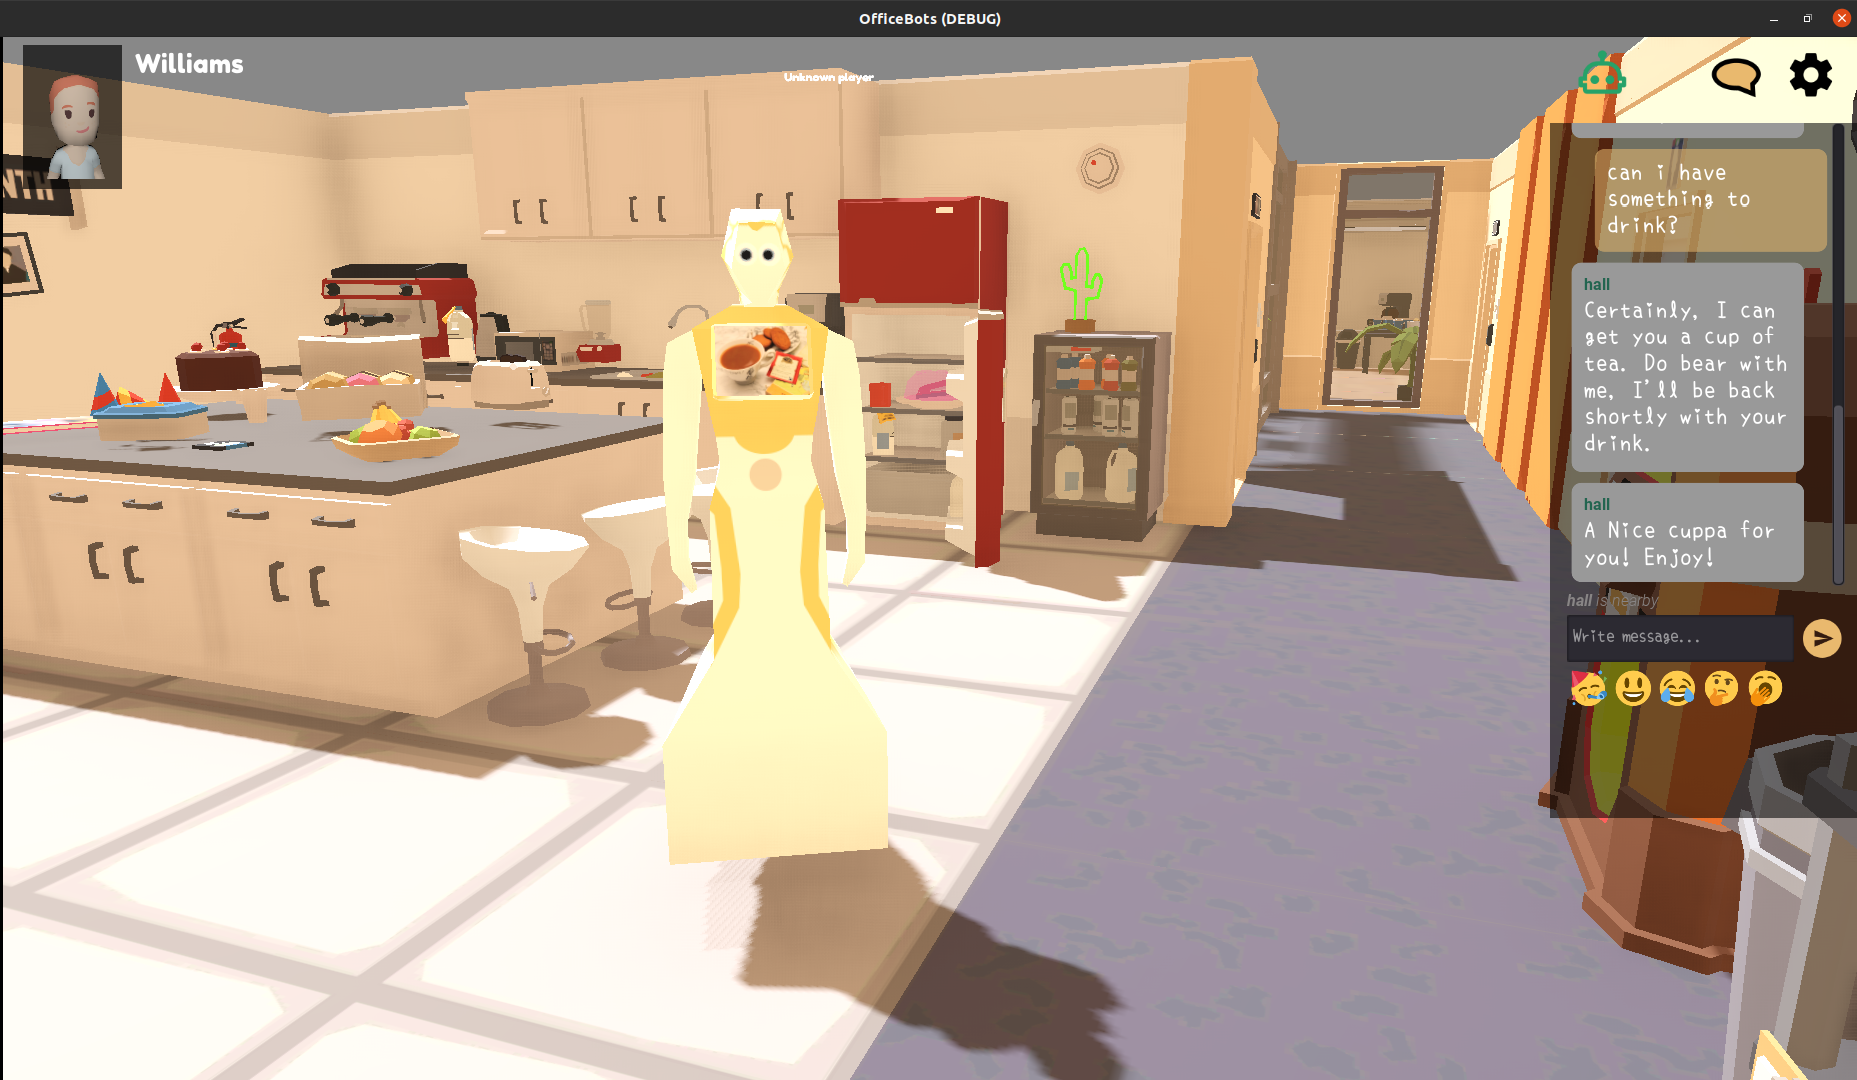
\includegraphics[width=\linewidth]{Chapter4/robot1.png}  
        \caption{Robot configured according to user input}
        \label{fig:figure1}
    \end{center}
\end{figure}

\begin{figure}
    \begin{center}
        \noindent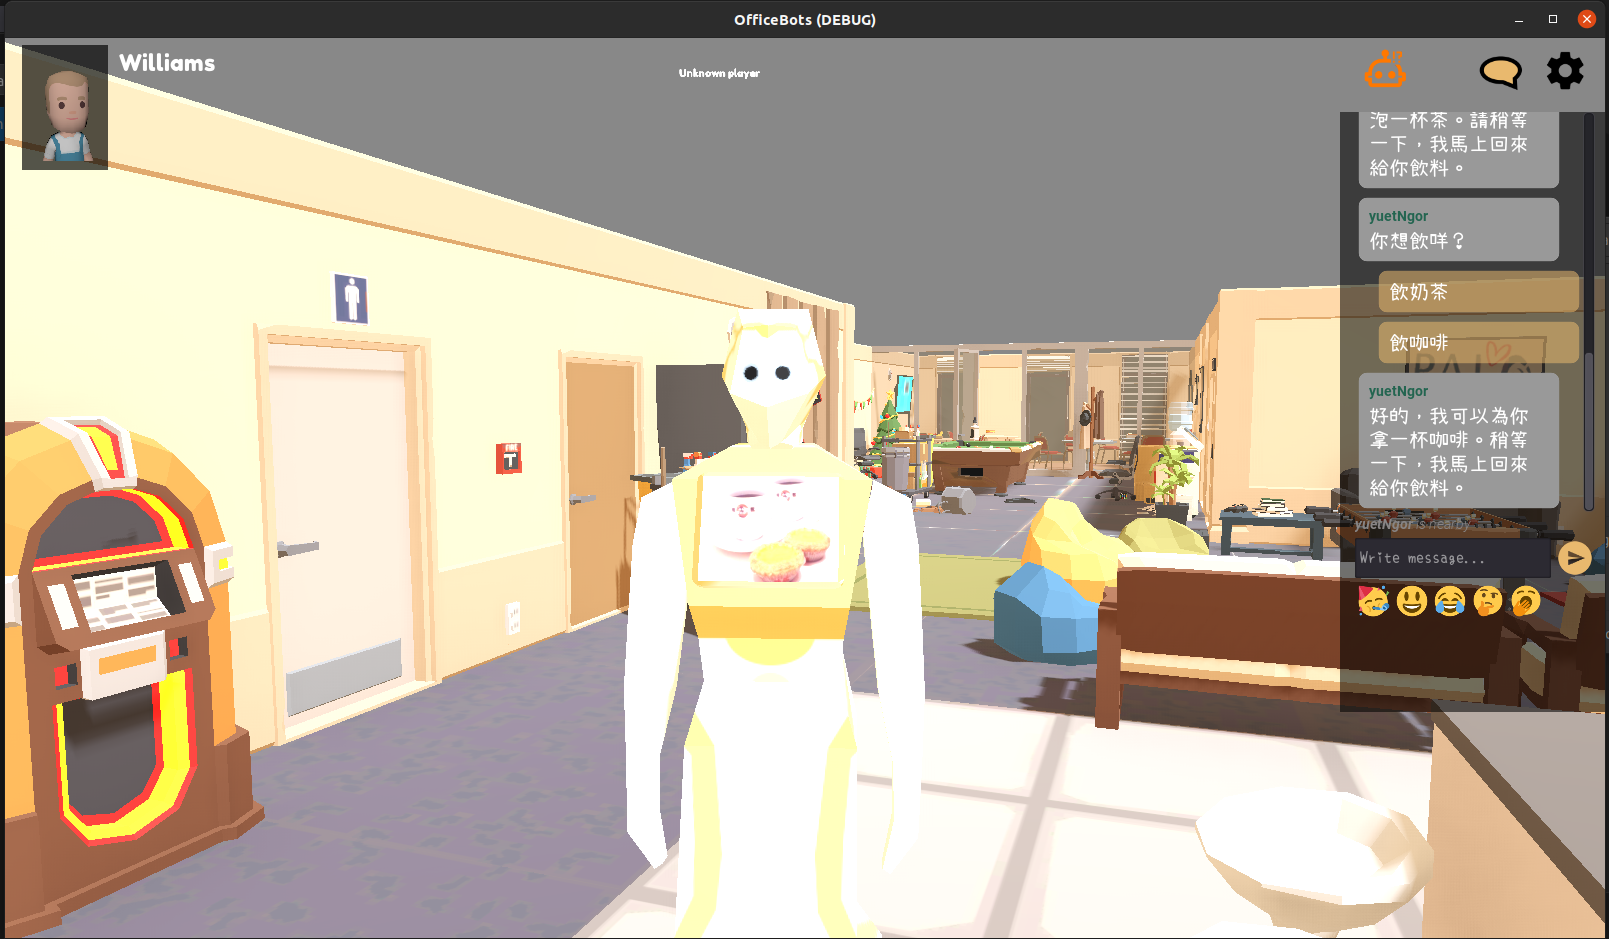
\includegraphics[width=\linewidth]{Chapter4/robot2.png}  
        \caption{An example of Chinese robot behaviour}
        \label{fig:figure1}
    \end{center}
\end{figure}

\subsubsection{Customization for Cultural Interactions}

The robots will be programmed with variances in language and behavioral cues based on cultural insights from the pre-experiment survey. Scenario variations will elicit and measure the adaptability of these culturally informed robot behaviors.


\section{Participant Recruitment}

The recruitment process targeted the selection of 15 participants, divided into three distinct cultural groups: Chinese, Hong Kong, and British. Each group consisted of five individuals, ensuring a balanced representation within the sample. This intentional sampling approach aimed to facilitate a focused examination of cultural behaviours and preferences within these culturally homogeneous cohorts.

\subsection{Recruitment Methodology}

Participants were recruited through a multifaceted approach that incorporated elements of both systematic sampling and snowball sampling techniques. While systematic sampling principles guided the structured identification and selection of individuals from the target cultural groups, personal networks and referrals were utilized through the application of snowball sampling.

\subsubsection{Systematic Sampling}

Systematic sampling principles were applied to ensure the comprehensive representation of the target cultural groups. This involved establishing clear criteria for participant selection and utilizing multiple recruitment channels to systematically identify eligible individuals. By adhering to systematic sampling principles, the study aimed to minimize bias and enhance the validity of the research findings.

\subsection{Snowball Sampling}

In addition to systematic sampling, snowball sampling techniques were utilized to capitalize on personal networks and referrals. Existing participants or contacts within the researcher's network may have referred additional individuals who met the study criteria. This facilitated the identification of potential participants who may not have been reached through traditional recruitment channels alone. While snowball sampling contributed to the expansion of the participant pool, it was integrated into the recruitment process alongside systematic sampling methods to ensure a comprehensive and diverse sample composition.

\section{Data Collection}

\subsubsection{Pre-Experiment Survey}

\textbf{Survey Design and Implementation:} Participants will first complete a pre-experiment survey designed to gather demographic information, cultural background, prior experiences with robots, and expectations for social robot interaction.

\subsubsection{Post-Experiment Survey and Feedback}

\textbf{User Study:} A post-experiment survey will collect immediate participant feedback about the robot interactions. This survey measures perceived cultural accuracy, engagement, and the overall acceptability of the robot behaviors.

\subsection{Ethical Considerations}

Prior to participation, all users will be briefed on the study's objectives, their role, and rights as participants, including confidentiality and the option to withdraw at any point without repercussion. The study will ensure that all ethical protocols and guidelines are rigorously followed.

\section{Experiment Procedure}

To rigorously evaluate the interactions between humans and culturally aware robots, this research includes a series of systematic experiments conducted within a controlled environment. This section describes the setup of these experiments, including the recruitment and briefing of participants, the execution of interaction scenarios, and the data collection methods used to record and assess the behavior of both the robots and the human subjects.

\subsection{Briefing and Instructions}

Upon recruitment, participants received a detailed briefing about the study's objectives and the nature of their involvement. They were assured of confidentiality and informed of their right to withdraw from the study at any time. Informed consent forms were obtained from all participants. Instructions were provided outlining how subjects should interact with the robots, emphasizing that they should behave as they would naturally in a real-world office setting. Additional clarifications and training were provided to ensure comfort with the OfficeBots simulation environment and to eliminate any unfamiliarity with the simulation software that might impact the experiment's outcome.

\subsection{Execution of Interaction Scenarios}

Interaction scenarios were designed to elicit culturally specific behaviors in both participants and robots. These scenarios included:

\begin{itemize}
    \item A greeting interaction, where the robot would approach and greet the participant using language cues pertinent to the participant's cultural context.
    \item A hospitality interaction, where the robot would offer a choice of drinks typical to the participant's culture.
    \item A personal space interaction, with the robot entering and maintaining a culturally appropriate distance during conversation.
\end{itemize}

The scenarios were conducted in random order to reduce the expectancy effect, and each participant went through interactions with all three culturally programmed robots to observe comparative responses.

\subsection{Ensuring Fidelity and Replicability}

All experiments were conducted in the same OfficeBots environment to ensure fidelity and to allow for data comparability. Precise documentation of software settings, robot behaviors, and participant interactions were maintained, promoting study replicability.

\subsection{Ethical Handling of Data}

Throughout the study, all data collection and analysis methods adhered strictly to ethical standards. Participant data was treated with the confidentiality, securely stored, and made accessible only to the research team. Personal identifiers were removed from all datasets to maintain anonymity in line with ethical research guidelines.


